\section{Abstrakte Architektur}
In diesem Dokument soll ein Transportsystem mit autonom agierenden Transportvehikeln (\emph{Robots}) entwickelt werden, welche sowohl Notfalltransporte für ein Krankenhaus (\emph{Hospital}) als auch Taxifahrten für Kunden eines Taxidienstes übernehmen. 

Fordert das \emph{Hospital} einen Krankentransport an, fährt der \emph{Robot} zur Abholung des Patienten an die angegebene Position, um ihn anschließend zum \emph{Hospital} zu bringen.
Einen Taxikunden holt der \emph{Robot} an dessen Position ab und bringt ihn anschließend zum gewünschten Ziel.

Dieser Entwurf basiert auf der in der Analyse erarbeiteten Spezifikation des Systems. Abbildung \ref{KomponentendiagrammAbstrakt} zeigt das abstrakte Komponentendiagramm.

\begin{figure}[H]
	\centering
	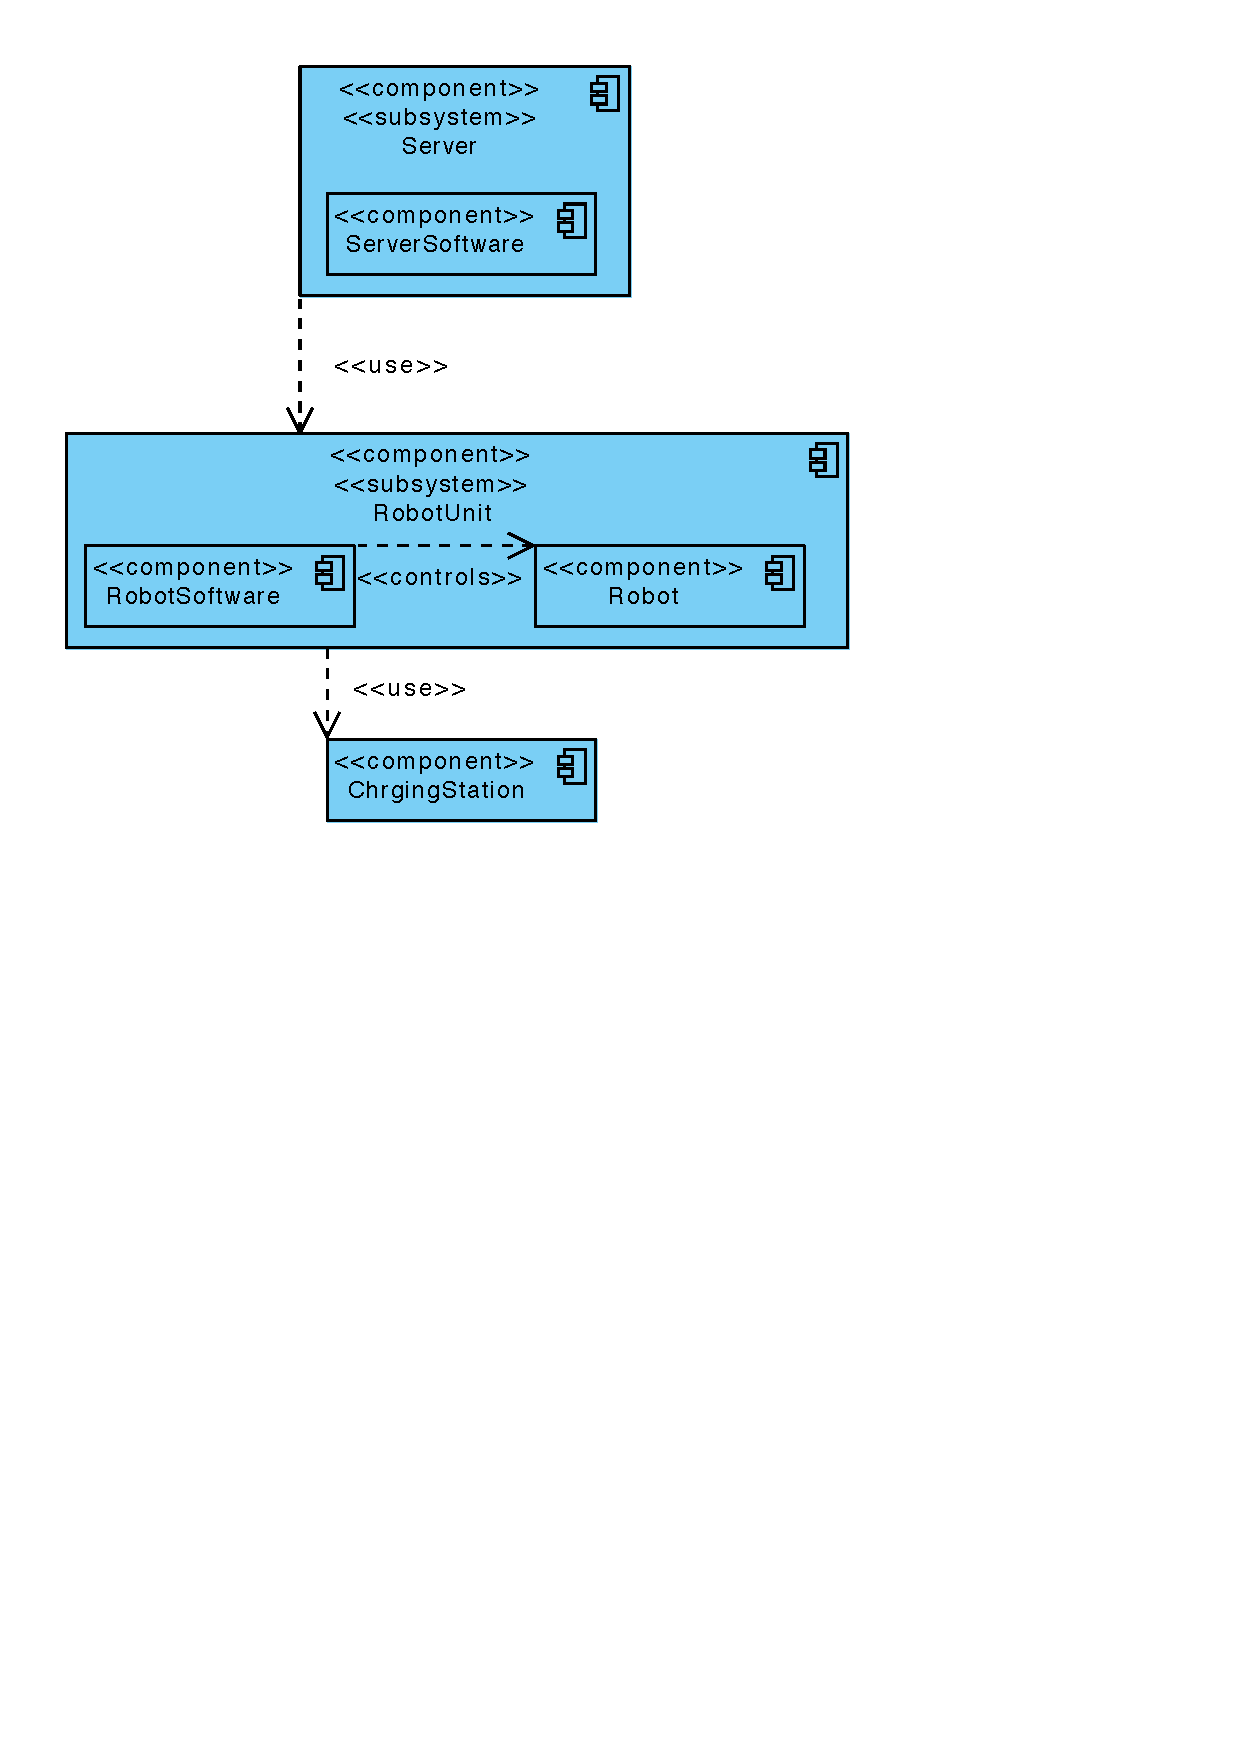
\includegraphics[width=0.8\textwidth]{img/AbstrakteArchitektur}
	\caption{Abstraktes Komponentendiagramm}
	\label{KomponentendiagrammAbstrakt}
\end{figure}

Die \emph{RobotUnit} bezeichnet die Kombination aus (durch die Spezifikation gegebenen) \emph{Robot} sowie der selbst erstellten \emph{RobotSoftware}.

In diesem Kapitel wird die im Rahmen der Analyse ermittelte Einteilung des Systems in Komponenten strukturiert dargestellt. 
Hierbei soll auch die Interaktion der Komponenten untereinander verdeutlicht werden.

\subsection{Server}

Der \emph{Server} nimmt Aufträge (\emph{Orders}) von Taxikunden und vom \emph{Hospital} entgegen und erstellt daraus intern \emph{Tasks}, die entweder direkt oder über eine Warteschlange an die \emph{RobotUnits} verteilt werden.

\subsubsection{ServerSoftware}

Die Komponente \emph{ServerSoftware} ist die auf dem \emph{Server} laufende Software. 
Sie greift auf die serverseitigen Subsysteme zu und stellt die zentrale Anlaufstelle f\"{u}r alle \emph{RobotUnits} sowie externe Akteure (\emph{Hospital} und \emph{TaxiApp}) dar.

\subsection{RobotUnit}

Die Komponente \emph{RobotUnit} sublimiert die \emph{RobotSoftware} und \emph{-Hardware} (Komponente \emph{Robot}) als eine Oberkomponente. 
Sie vereint alle Hard- und Softwareinterfaces dieser Komponenten und leitet die ein- und ausgehenden Nachrichten der \emph{RobotSoftware} an den \emph{Server} weiter. 
Sie dient somit als \"{u}bergeordnete Schnittstelle f\"{u}r die Kommunikation.

\subsubsection{RobotSoftware}

Die \emph{RobotSoftware} steuert den \emph{Robot} an und verwertet seine Sensordaten, um die Fahrlogik zu implementieren. Außerdem kommuniziert sie mit dem \emph{Server}, um diesen über Kollisionen oder das Erreichen eines Zieles zu informieren.

\subsubsection{Robot}

Die Komponente \emph{Robot} ist durch die Spezifikation gegeben und beinhaltet alle hardwaretechnischen Funktionen des \emph{Robots}. 
Dazu geh\"{o}rt die \emph{IDrive} Schnittstelle, die interne Sensorik sowie die \emph{IBattery}.
